\part{Einleitung}
\label{part:intro}

\begin{frame}[fragile]{}
Einleitung!
\end{frame}

\part{HoloLens}
\label{part:hololens}
\begin{frame}[fragile]{}
\begin{figure}[h!]
	\centering
	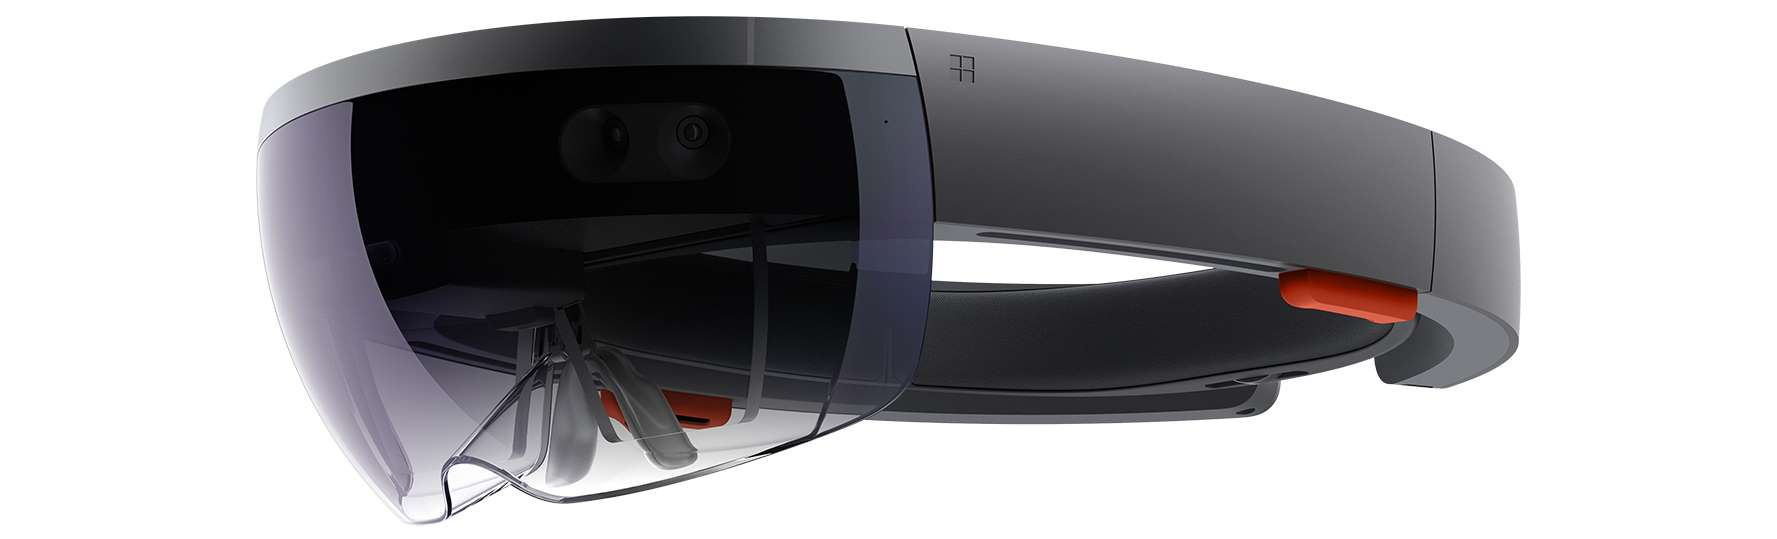
\includegraphics[width=0.7\textwidth]{images/hololens.jpg}
\end{figure}
\begin{itemize}
	\pause
	\item \textit{Mixed Reality} Device
	\pause
	\item Projeziert virtuelle Objekte in das Sichtfeld des Nutzers
	\pause
	\item Nutzer bewegt sich simultan durch reale und virtuelle Szene
	\pause
	\item Genaue Bestimmung von Position und Ausrichtung im Raum durch Sensoren: \textit{Inside-Out-Tracking}
\end{itemize}	
\end{frame}

\part{State of the Art}
\label{part:sota}

\begin{frame}[fragile]{HoloLens in der Physik}
%\begin{itemize}
%	\item 
%	\item Darstellung des Wärmeprofiles bei einem erhitzten Metallstab \cite{Strzys18}	
%\end{itemize}

\begin{figure}
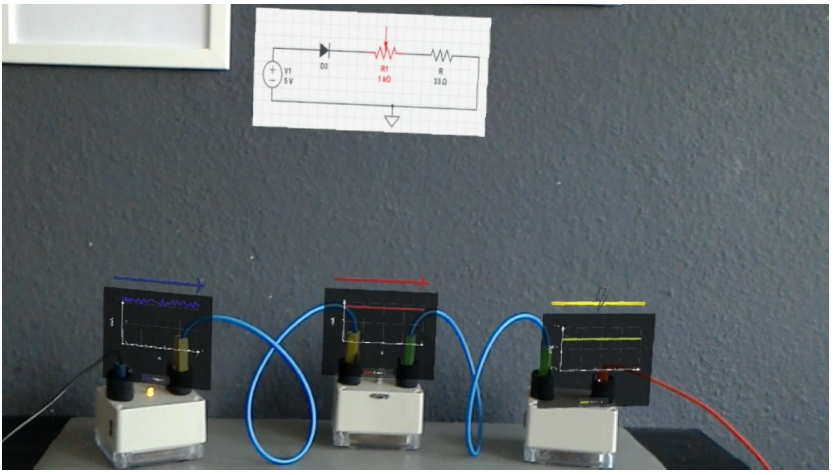
\includegraphics[width=0.45\textwidth]{images/Amiraslanov18.png}
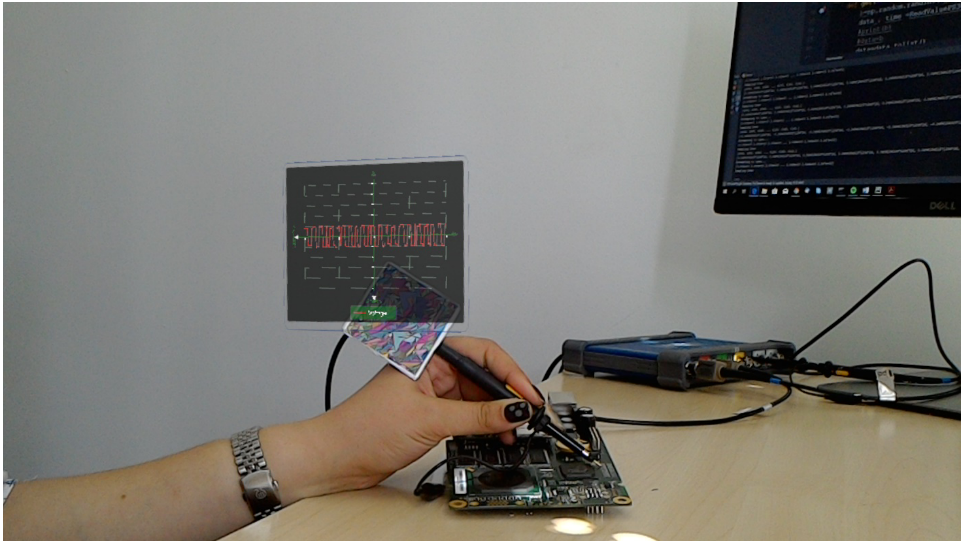
\includegraphics[width=0.45\textwidth]{images/Javaheri18.png}
\begin{center}
\vspace{0.05cm}
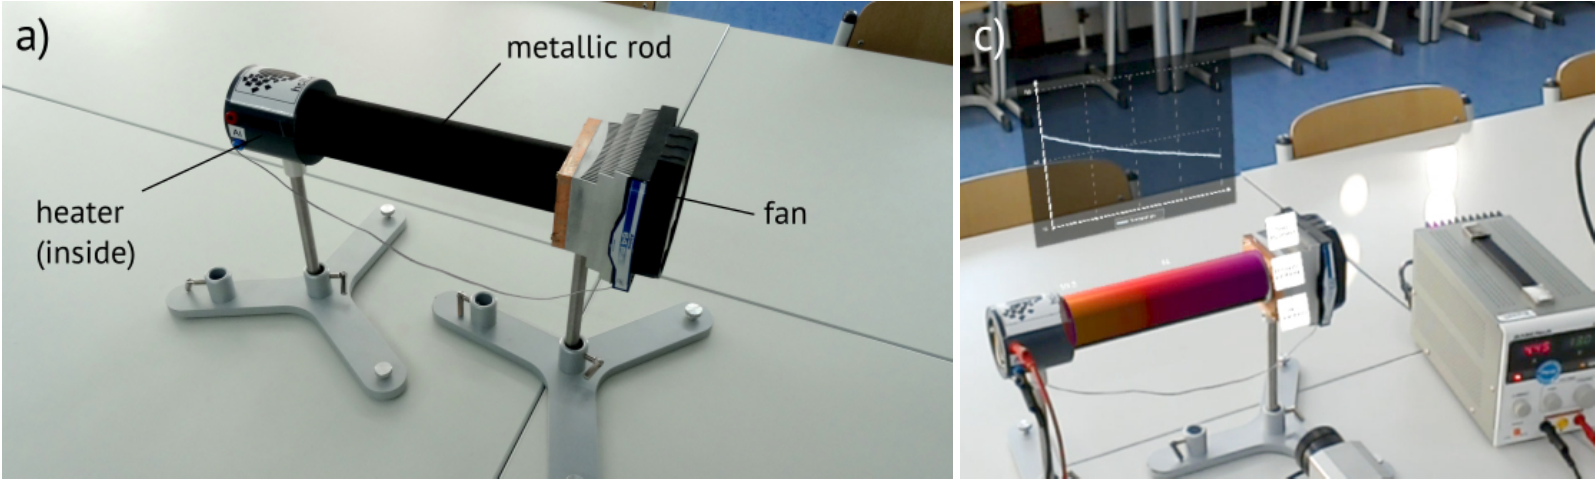
\includegraphics[width=0.9\textwidth]{images/Strzys18.png}	
\end{center}
\setlength{\abovecaptionskip}{5pt plus 5pt minus 2pt}
\caption*{Oben Links: \citep{Amiraslanov18}, Oben Rechts: \cite{Javaheri18}, Unten: \cite{Strzys18}}
\end{figure}

\end{frame}

\begin{frame}[fragile]{Mixed Reality in der Physik}

\begin{figure}
	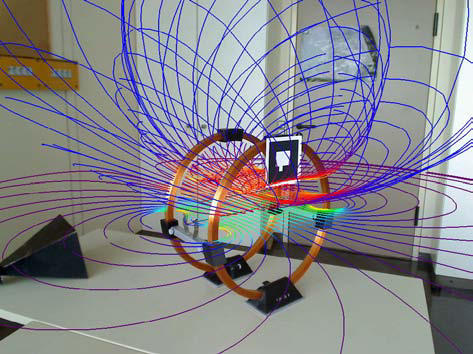
\includegraphics[width=0.35\textwidth]{images/Buchau09.jpg}
	\hspace{0.05cm}
	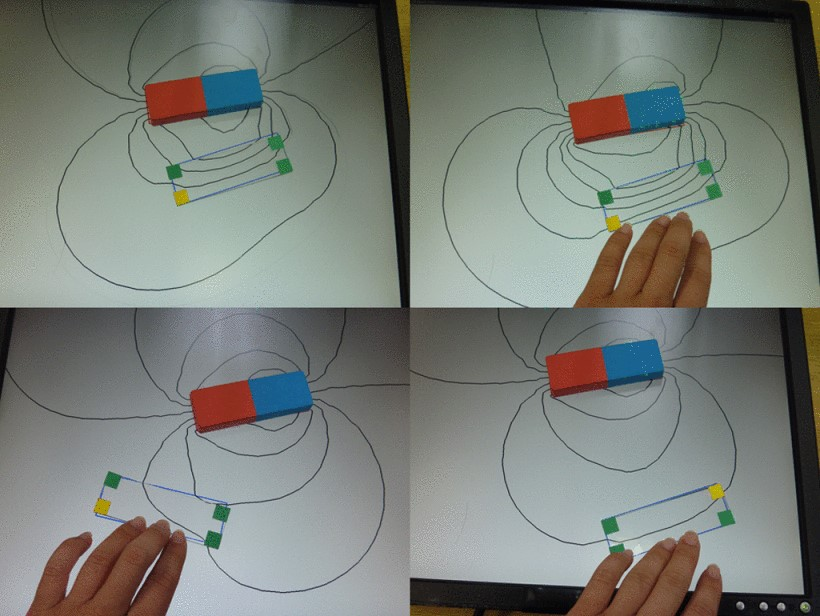
\includegraphics[width=0.35\textwidth]{images/Matsutomo13.jpg}

%	\centering
	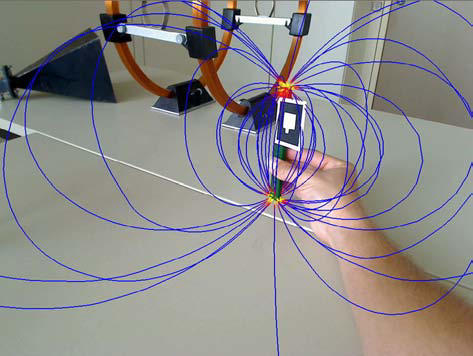
\includegraphics[width=0.35\textwidth]{images/Buchau09_Magnet.jpg}
	\hspace{0.05cm}
	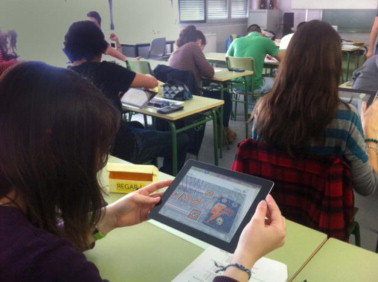
\includegraphics[width=0.35\textwidth]{images/Ibanez14.jpg}

	\setlength{\abovecaptionskip}{5pt plus 5pt minus 2pt}
	\caption*{Links: \citep{Buchau09}, Rechts Oben: \cite{Matsutomo13}, Rechts Unten: \cite{Ibanez14}}
\end{figure}

\end{frame}

\part{Anwendungsfall: Helmholtz-Spulen}
\label{part:physics}

\begin{frame}[fragile]{}
Probleme und Ziele!

\end{frame}

\part{Problemstellung und Ziele}
\label{part:golas}

\begin{frame}[fragile]{}
Probleme und Ziele!

\end{frame}

\begin{frame}[fragile]{Anforderungen}
\begin{itemize}
	\item Magnetfeld von Erde und Spule
	\subitem Stärke
	\subitem Richtung
	\subitem Homogenität
	\subitem Inhomogenität am Rand der Spule andeuten (Optional)
	\item Stromfluss durch die Spule
	\subitem Richtung
	\subitem Kennzeichnung von Plus und Minus
	\subitem Stärke (Optional)
	\item Kompass
	\item Weitere Informationen zum Versuchsaufbau
\end{itemize}
\end{frame}

\part{Design}
\label{part:design}

\begin{frame}[fragile]{}
Design
\end{frame}

\part{Umsetzung und Ausblick}
\label{part:practice}

\begin{frame}[fragile]{}
ASDF
\end{frame}